Following the integration of updated high temperature opacities detailed in \S
\ref{sec:p1}, we will investigate using the observed color and magnitude range
of the Jao Gap to age-date coeval populations within the solar neighboorhood.

While low-mass stars provide the majority of the fitting points for isochrones
when estimating ages of clusters, due to the very slow variations in
observables during main sequence evolution, it remains challenging to measure
precise and accurate ages for low mass field stars \citep{Soderblom2010,
Veyette2018, Kiman2021}. Due to the extremely high density of isochrones near
the Zero-Age Main Sequence, isochrone age estimates for K and M dwarfs can have
uncertaninties as high as 50 \% \citep{Lu2021}. As a result of these high isochrone age
uncertaninties other methods of dating non-cluster populations have been
developed, including age-calibrated rotation-activity relations
\citep[e.g.][]{Kiman2021} and gyro-kinematic age-dating
\citep[e.g.][]{Lu2021}. In this chapter of the thesis we will present
calibrations of Jao Gap location to serve as an additional age-dating method.

Preliminary modeling we have done, along with past literature
\citep[e.g.][]{Jao2018,Jao2020,Feiden2021,Mansfield2021} demonstrates that the
Jao Gap is expected to migrate along the main sequence as a population of stars
age. Our modeling indicates that stellar populations younger than $\sim 2 Gyr$
do not show a gap. However, once the gap forms it will migrate towards brighter
portions of the CMD with age until a population age of $\sim 8$ Gyr.

For this proposal we do not perform any rigorous statistical testing of whether
the differences in theoretical Jao Gap location could be discrimated between in
observational data; instead, choosing to save that element of the research for
thesis work proper. However, we do perform a qualitative test of the visual
distinguisability of the Jao Gap location for two sample sizes --- 500 and 1000
stars (Figure \ref{fig:JGTTE}).

\begin{equation}\label{eqn:IMF}
	\xi(m) = \xi_{0}\left(\frac{m}{M_{\odot}}\right)^{-2.68\pm0.09}
\end{equation}

We evolve models over an extremely finely sampled mass grid centered at the
theoretical Jao Gap location for a GS98 solar composition population of stars.
We then adopt the \citep{Sollima2019} IMF between 0.1 and 1 $M_{\odot}$
(Equation \ref{eqn:IMF}) to sample these evolved models. Model surface
gravities, effective temperatures, and luminosities are transformed into Gaia
magnitudes using bolometric correction tables provided by
ESA\footnote{\url{https://gea.esac.esa.int/archive/documentation/GDR2/Data\_processing/chap\_cu5pho/sec\_cu5pho\_calibr/ssec\_cu5pho\_calibr\_extern.html}}
and color-code provided by Dotter. Uncertainty is injected by first
transforming $G$, $BP$, and $RP$ flux and flux uncertaninty measurments for all
stars Gaia observed within 10pc to magnitude and magnitude uncertaninties. Flux
errors do not transform into symetric magnitude errors; however, for small
uncertainties the transformation may be approximated as symmetric (Equations
\ref{eqn:fluxerr2magerr} \& \ref{eqn:sigfluxerr2magerr}).

\begin{equation}\label{eqn:fluxerr2magerr}
	M_{x} = -2.5\log_{10}(I_{x}) + ZP_{x}
\end{equation}
\begin{equation}\label{eqn:sigfluxerr2magerr}
	\sigma_{x} = \left(\frac{1.086\sigma_{I_{x}}}{I_{x}}\right)^{2} + ZP_{\sigma_{I_{x}}}^{2}
\end{equation}

Where $x$ is the band of interest, $I_{x}$ is the measured flux in that band,
and $ZP_{x}$ is the zero point offset in \texttt{VEGAMAG}. Following this
transformation, we fit a second-order polynominal to the magnitude error v.s.
magnitude for each band. This polynominal gives an approximation of the mean
uncertaninty for a given magnitude. For each point sampled from the IMF and set
of evolved models we add a sample from a normal distribution centered at 0 and
with a standard deviation equal to the evaluation of the optimized quadradic at
that point's magnitude.

Figure \ref{fig:JGTTE} Panels A and B show (1 Gyr) do not show any visible Jao
Gap; whereas, Panels C, D, E, and F all do. Moreover, the location of the Gap
visiblly shifts to lower magnitudes from 3 Gyr to 6 Gyrs. Note that this shift
is apparent in CMDs with both 1000s stars and those with 500 stars. In fact,
visually, this shift is clear with CMDs containing as few as 100 stars within
the modeled color range. Querying Gaia DR3 over this same color range yields
245 sources within 100 lightyears.  Obviously, a simple visual identification
is prone to confirmation bias; however, we believe that these results are
sufficent to warrant a future, more rigorous, study.


\begin{figure}
	\centering
	\includegraphics[width=0.8\textwidth]{src/Figures/JaoGapTheoreticalTimeEvolution.pdf}
	\caption{Populations synthesis results for a mass range surrounding the
	theoretical location of the Jao Gap at 3 population ages and with different
	sample sizes. The superimposed color map is derived from a Gaussian
	kernel-density-estimation run on the displayed points. This is included to
	better illustrate the gap location.}
	\label{fig:JGTTE}
\end{figure}

Identifying the Jao Gap's location one half of this work, the other half is to
tie these shifts in gap location to established age proxies --- that is we need
to calibrate the Jao Gap's age sensitivity. We propose to model a population of
stars of various ages and mettalicities sampled from the solar neighboorhood.
Each of these stars will be assigned kinematics --- again sampled from
empirical distributions \citep[Figure \ref{fig:LuKde},][]{Lu2021}. We will then
extract kinematically derived ages from this population and use these to
segregate stars into rough age bins. Finally, we will measure if difference in
Jao Gap locations are statistically distinquishable between these rough age
bins.

\begin{figure}
	\centering
	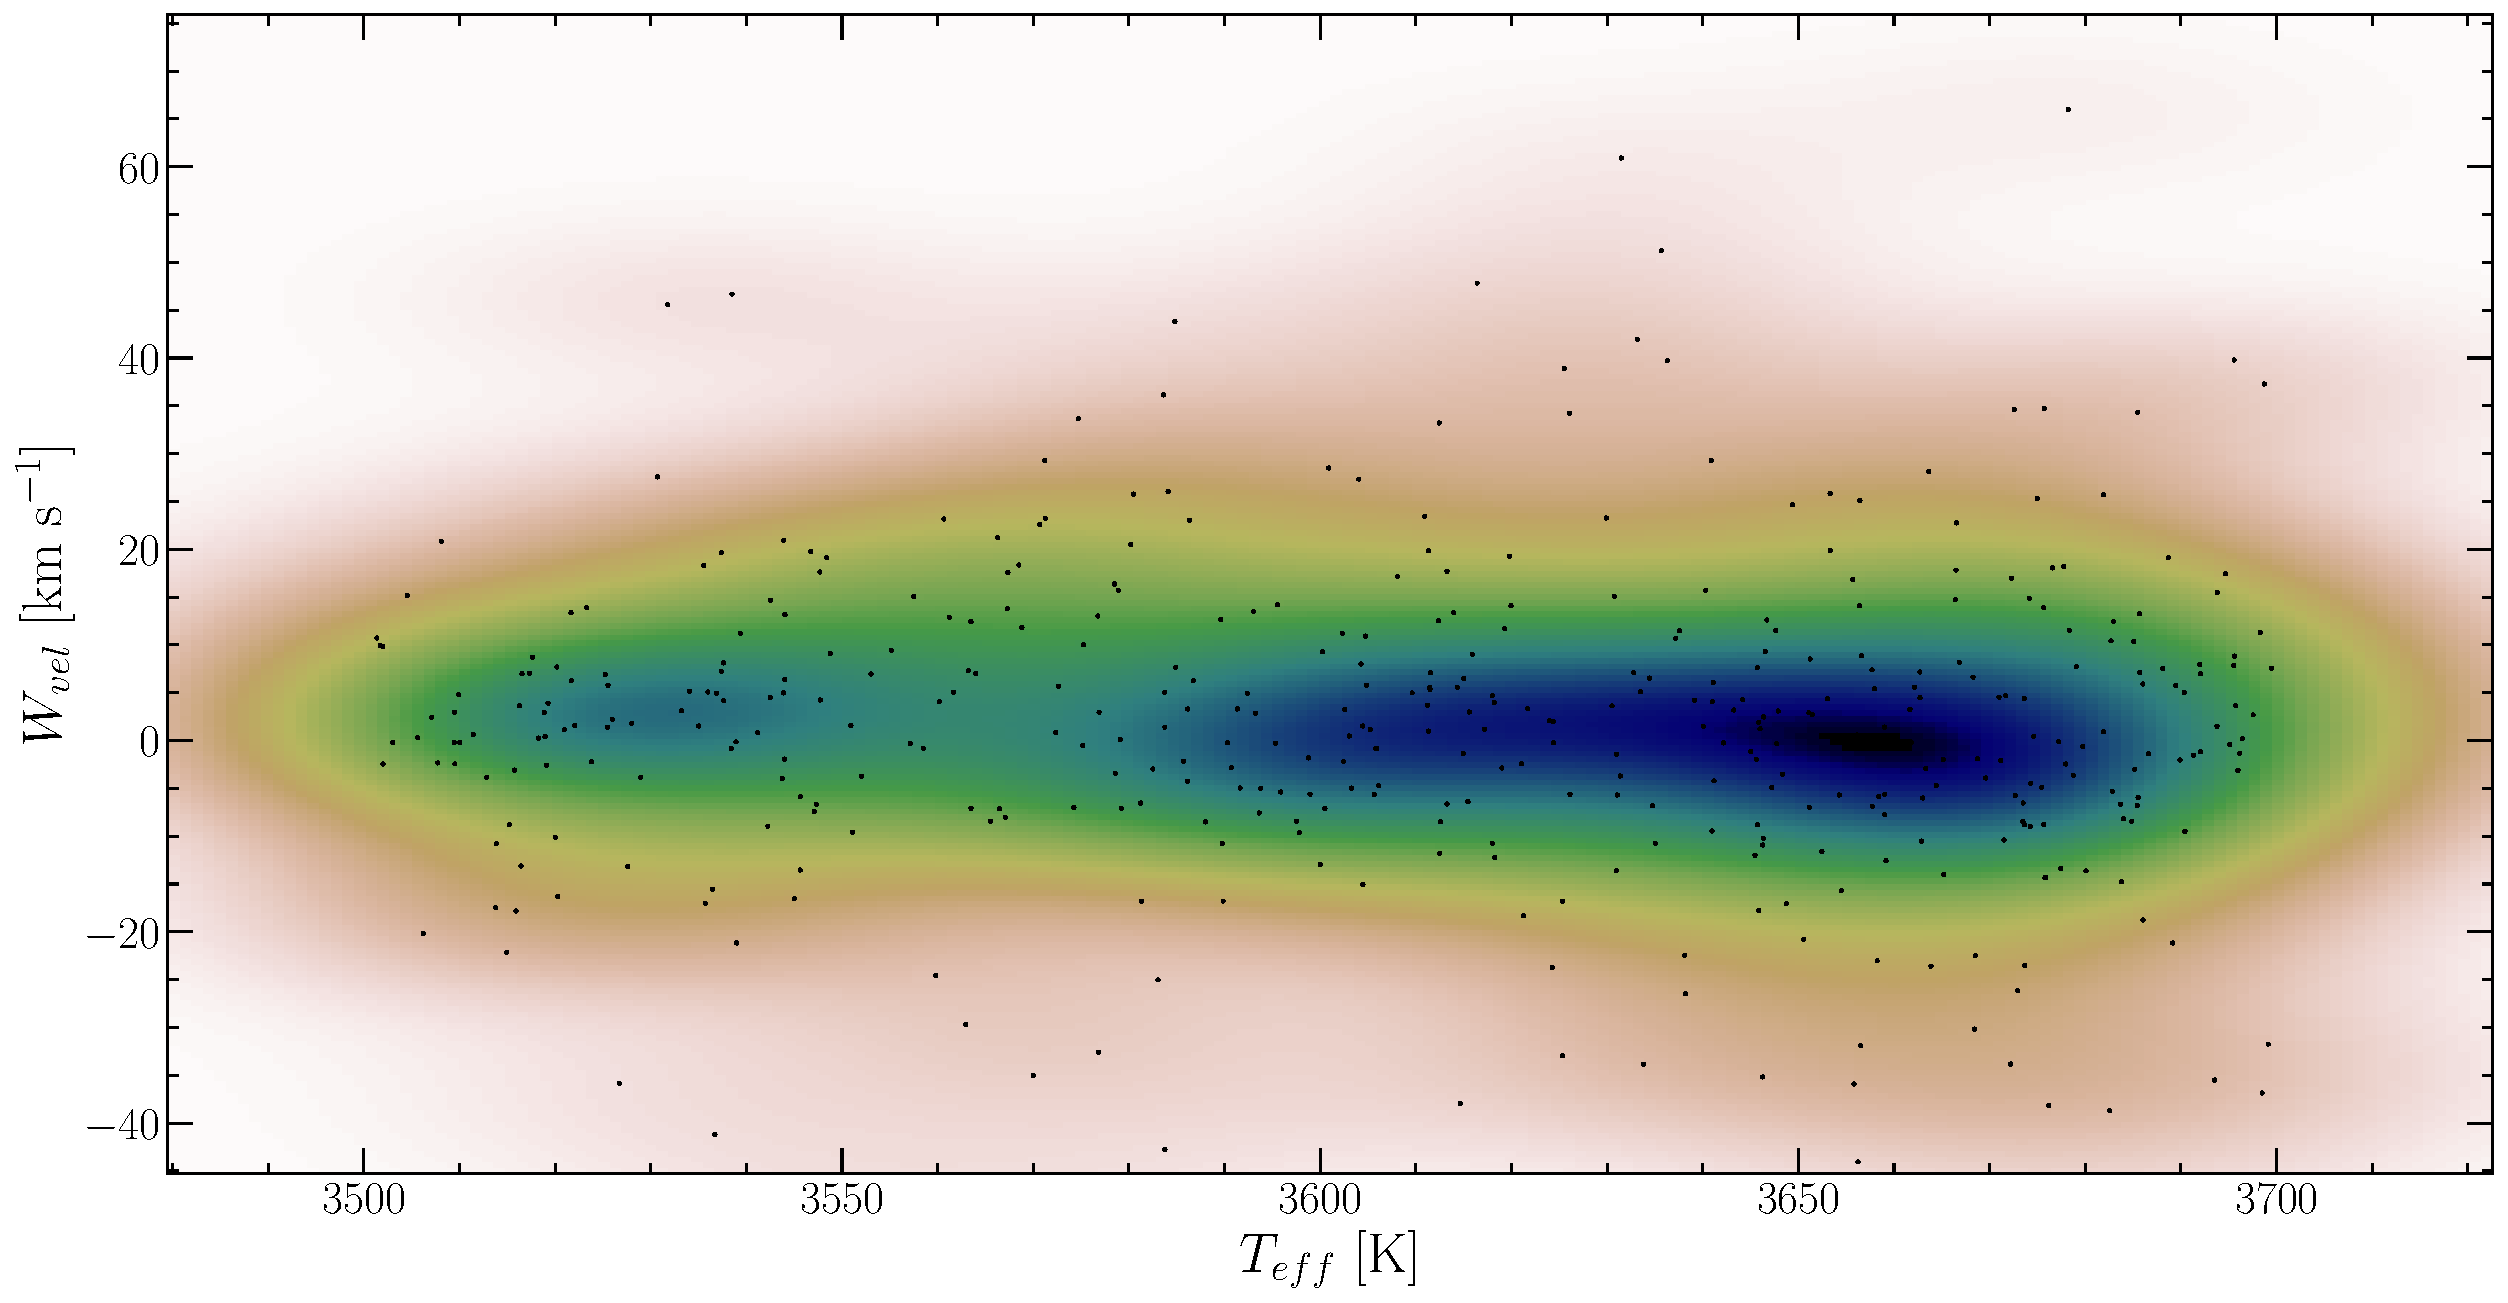
\includegraphics[width=0.75\textwidth]{src/Figures/LuEtAlKDE.pdf}
	\caption{Kernel Density Estimation function of the gyro-kinematically
	inferred velocity vs. effective temperature. This sample is selected from
	\citet{Lu2021} and cut between $T_{eff} < 3800$ K and $T_{eff} > 3500$ K,
	roughly the temperature range of the Jao Gap. {\color{red}[Make this a hist?]}}
	\label{fig:LuKde}
\end{figure}
